\documentclass[12pt]{ximera}
\title{Final Exam (Fall 2023)}
\begin{document}
\begin{abstract}
An archived cumulative final: Plurality-with-Elimination with a tie, a Pairwise Comparisons cycle, lone-divider on a cake, sealed bids, Banzhaf and Shapley-Shubik power, Hamilton and Jefferson apportionment, and dominance and saddle points.
\end{abstract}
\maketitle

\section*{Final Exam (Fall 2023)}

\begin{problem}
Questions 1 and 2 use the following preference schedule.
\begin{center}
\begin{tabular}{c|ccccc}
Number of voters & 10 & 9 & 6 & 4 & 2\\\hline
1st & D & C & A & B & B\\
2nd & B & D & C & C & D\\
3rd & C & A & B & A & C\\
4th & A & B & D & D & A
\end{tabular}
\end{center}

\begin{prompt}
\textbf{1.} Use Plurality-with-Elimination, breaking ties by coin toss. Who wins, and
who comes second?

1st $\answer{C}$ \quad 2nd $\answer{D}$
\begin{feedback}
Round 1: D $10$, C $9$, A $6$, B $6$. A and B tie for last.
\begin{itemize}
\item Eliminate A first: its $6$ voters go to C (C $15$). Then B ($6$) goes out: $4$ votes
      to C and $2$ to D, so C $19$, D $12$. Ranking C, D, B, A.
\item Eliminate B first: C $13$, D $12$, A $6$. Then A goes out and C reaches $19$.
      Ranking C, D, A, B.
\end{itemize}
Either way C wins and D is second.
\end{feedback}
\end{prompt}

\begin{prompt}
\textbf{2.} Using Pairwise Comparisons, how many points does each candidate get?

A $\answer{0}$ \quad B $\answer{2}$ \quad C $\answer{2}$ \quad D $\answer{2}$

\smallskip
Is there a Condorcet candidate?
\begin{multipleChoice}
\choice{Yes, B}
\choice{Yes, C}
\choice{Yes, D}
\choice[correct]{No}
\end{multipleChoice}
\begin{feedback}
B beats A $16$--$15$; C beats A $25$--$6$; D beats A $21$--$10$; B beats C $16$--$15$;
D beats B $19$--$12$; C beats D $19$--$12$. B, C, D tie for first with $2$ points each,
in a cycle (B beats C, C beats D, D beats B), so there is no Condorcet candidate.
\end{feedback}
\end{prompt}
\end{problem}

\begin{problem}
A cake has three equal parts: red velvet (V), carrot (C), and strawberry (S). The whole
cake is worth \$24.
\begin{center}
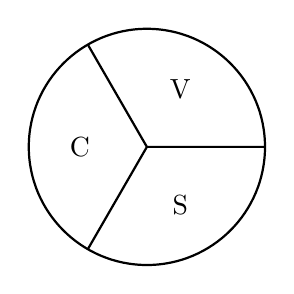
\begin{tikzpicture}
\draw[thick] (0,0) circle (1.5);
\draw[thick] (0,0) -- (0:1.5) (0,0) -- (120:1.5) (0,0) -- (240:1.5);
\node at (60:0.85) {V}; \node at (180:0.85) {C}; \node at (300:0.85) {S};
\end{tikzpicture}
\end{center}
Alicia, Billy, Charlie, and David divide it with the lone-divider method, with David as
divider. David likes C twice as much as V, and S three times as much as V.

\begin{prompt}
\textbf{(a)} What is the red velvet part worth to David? $\$\answer{4}$
\begin{feedback}
With $C=2V$ and $S=3V$, $V+2V+3V=24$, so $V=4$ (and $C=8$, $S=12$).
\end{feedback}
\end{prompt}

\begin{prompt}
\textbf{(b)} How much should each of the four shares be worth to him? $\$\answer{6}$
\end{prompt}

\begin{prompt}
\textbf{(c)} David cuts from the center to the edge, starting along the line between V and
S. His first share is all of V plus part of C. What fraction of C goes into $s_1$, and how
is S split?

Fraction of C in $s_1$: $\answer{1/4}$ \quad Fraction of S in each of $s_3$ and $s_4$:
$\answer{1/2}$
\begin{feedback}
$s_1$ needs $\$2$ beyond V's $\$4$, and C is worth $\$8$, so $\frac14$ of it:
$s_1=V+\frac14C$. Then $s_2=\frac34C$ (worth $\$6$), and $s_3=s_4=\frac12S$.
\begin{center}

\includegraphics[width=2.2in]{cakeShares.png}
\end{center}
\end{feedback}
\end{prompt}

\begin{prompt}
\textbf{(d)} Alicia likes C and V equally, but likes S twice as much as C. Which of
David's shares are acceptable to her?
\begin{selectAll}
\choice[correct]{$s_1$}
\choice{$s_2$}
\choice[correct]{$s_3$}
\choice[correct]{$s_4$}
\end{selectAll}
\begin{feedback}
To Alicia, $V=C=6$ and $S=12$. So $s_1=6+\frac14\cdot6=7.5$, $s_2=4.5$, and $s_3=s_4=6$.
Acceptable means at least $\$6$.
\end{feedback}
\end{prompt}
\end{problem}

\begin{problem}
Alex, Bill, and Charli divide their late aunt's paintings by sealed bids (in thousands of
dollars).
\begin{center}
\begin{tabular}{r|rrr}
 & Alex & Bill & Charli\\\hline
Monet & 150 & 180 & 160\\
D\"urer & 260 & 400 & 200\\
Van Gogh & 380 & 300 & 240\\
Picasso & 110 & 140 & 120
\end{tabular}
\end{center}

\begin{prompt}
\textbf{(a)} Who gets each painting?

Monet $\answer{Bill}$ \quad D\"urer $\answer{Bill}$ \quad Van Gogh $\answer{Alex}$ \quad
Picasso $\answer{Bill}$
\end{prompt}

\begin{prompt}
\textbf{(b)} Initial settlement (positive = pays): Alex $\answer{80}$ \quad Bill
$\answer{380}$ \quad Charli $\answer{-240}$
\begin{feedback}
Totals $900$, $1020$, $720$; fair shares $300$, $340$, $240$. Alex's Van Gogh is $80$ over;
Bill's three paintings ($720$) are $380$ over; Charli receives $240$.
\end{feedback}
\end{prompt}

\begin{prompt}
\textbf{(c)} Surplus: $\answer{220}$ thousand
\end{prompt}
\end{problem}

\begin{problem}
Four players A, B, C, D use the weighted voting system $[10:6,5,4,3]$.

\begin{prompt}
\textbf{(a)} How many winning coalitions are there? $\answer{7}$
\end{prompt}

\begin{prompt}
\textbf{(b)} Banzhaf power distribution, as fractions: A $\answer{5/12}$, B $\answer{1/4}$,
C $\answer{1/4}$, D $\answer{1/12}$
\begin{feedback}
Winning coalitions, critical players underlined:
$\set{\underline A,\underline B}$, $\set{\underline A,\underline C}$,
$\set{\underline A,B,C}$, $\set{\underline A,\underline B,D}$,
$\set{\underline A,\underline C,D}$, $\set{\underline B,\underline C,\underline D}$,
$\set{A,B,C,D}$. Critical counts $5,3,3,1$, total $12$.
\end{feedback}
\end{prompt}
\end{problem}

\begin{problem}
The weighted voting system $[11:6,5,4,3]$ has players A, B, C, D.

\begin{prompt}
\textbf{(a)} How many sequential coalitions are there? $\answer{24}$
\end{prompt}

\begin{prompt}
\textbf{(b)} Which of these sequential coalitions have A (weight $6$) \emph{not}
pivotal?
\begin{selectAll}
\choice[correct]{$\seq{B,C,D,A}$}
\choice[correct]{$\seq{D,A,B,C}$}
\choice{$\seq{B,A,C,D}$}
\choice{$\seq{C,D,A,B}$}
\end{selectAll}
\begin{feedback}
In $\seq{B,C,D,A}$ the others already total $12\ge11$ before A arrives. In
$\seq{D,A,B,C}$, D and A total only $9$, and B is pivotal. In $\seq{B,A,C,D}$, A brings $5$
up to $11$; in $\seq{C,D,A,B}$, A brings $7$ up to $13$.
\end{feedback}
\end{prompt}

\begin{prompt}
\textbf{(c)} A and B each have pivotal count $8$, and C and D each have $4$. Find the
Shapley-Shubik indices.

A $\answer{1/3}$ \quad C $\answer{1/6}$
\begin{feedback}
$\frac8{24}=\frac13$ and $\frac4{24}=\frac16$. (The original exam gave C a count of $6$,
but a full count gives $8,8,4,4$.)
\end{feedback}
\end{prompt}
\end{problem}

\begin{problem}
A university apportions $50$ faculty senate seats among its six colleges by
undergraduate enrollment (in hundreds), using Hamilton's method.
\begin{center}
\begin{tabular}{r|rrrrrr|r}
College & Agric. & Business & Design & Engin. & Health & Lib.\ Arts & Total\\\hline
Enrollment & 51 & 83 & 43 & 25 & 41 & 37 & 280
\end{tabular}
\end{center}

\begin{prompt}
\textbf{(a)} Standard divisor: $\answer{5.6}$
\end{prompt}

\begin{prompt}
\textbf{(b)} Hamilton apportionment: Agric.\ $\answer{9}$, Business $\answer{15}$,
Design $\answer{8}$, Engin.\ $\answer{4}$, Health $\answer{7}$, Lib.\ Arts $\answer{7}$
\begin{feedback}
Quotas: $9.11$, $14.82$, $7.68$, $4.46$, $7.32$, $6.61$. The lower quotas
$9,14,7,4,7,6$ total $47$; the $3$ extra seats go to Business ($0.82$), Design ($0.68$),
and Liberal Arts ($0.61$).
\end{feedback}
\end{prompt}
\end{problem}

\begin{problem}
A city allocates $10$ polling stations to three wards by Jefferson's method.
\begin{center}
\begin{tabular}{r|ccc}
Ward & A & B & C\\\hline
Population & 210 & 200 & 390
\end{tabular}
\end{center}

\begin{prompt}
\textbf{(a)} Standard divisor $\answer{80}$; standard quotas A $\answer{2.625}$,
B $\answer{2.5}$, C $\answer{4.875}$
\end{prompt}

\begin{prompt}
\textbf{(b)} Jefferson apportionment: A $\answer{3}$, B $\answer{2}$, C $\answer{5}$
\begin{feedback}
Any divisor from about $66.67$ up to $70$ works; at $d=70$ the quotas are $3.00$, $2.86$,
$5.57$.
\end{feedback}
\end{prompt}
\end{problem}

\begin{problem}
Player A's strategies are the rows and B's the columns; entries are payments from B to A.
\[
\begin{bmatrix} 5 & 10 & 3 & 6\\ 8 & 12 & 7 & 9\\ -2 & 1 & 4 & 3 \end{bmatrix}
\]

\begin{prompt}
\textbf{(a)} Which strategy for A dominates A's first strategy? Row $\answer{2}$
\begin{feedback}
Every entry of row 2 exceeds the matching entry of row 1.
\end{feedback}
\end{prompt}

\begin{prompt}
\textbf{(b)} Which strategy for B dominates B's second strategy? Column $\answer{1}$
\begin{feedback}
B wants small payoffs, and column 1 ($5,8,-2$) is smaller than column 2 ($10,12,1$) in
every row.
\end{feedback}
\end{prompt}

\begin{prompt}
\textbf{(c)} The saddle point is in row $\answer{2}$, column $\answer{3}$, with value
$\answer{7}$.
\begin{feedback}
The row minimums are $3,7,-2$, with maximum $7$; the column maximums are $8,12,7,9$, with
minimum $7$.
\end{feedback}
\end{prompt}
\end{problem}

\end{document}
